% https://iitdbgroup.github.io/ProvenanceWeek2021/tapp.html

\documentclass[letterpaper,twocolumn,10pt]{article}
\usepackage{usenix-2020-09}

% to be able to draw some self-contained figs
\usepackage{tikz}
\usepackage{amsmath}
\usepackage{tabu}

% inlined bib file
% \usepackage{filecontents}
% 
% %-------------------------------------------------------------------------------
% \begin{filecontents}{\jobname.bib}
% %-------------------------------------------------------------------------------
% %
% %
% %
% \end{filecontents}

%-------------------------------------------------------------------------------
\begin{document}
%-------------------------------------------------------------------------------

% don't want date printed
\date{}

% make title bold and 14 pt font (Latex default is non-bold, 16 pt)
\title{\Large \bf An industrial provenance capability based on PROV for broad ranging IT projects including AI: Application Track}

% for single author (just remove % characters)
\author{
{\rm Nicholas J. Car}\\
SURROUND Pty Ltd \&\\
Australian National University\\
\href{mailto:nicholas.car@surroundaustralia.com}{nicholas.car@surroundaustralia.com} 
\and
{\rm Robert A. Atkinson}\\
SURROUND Pty Ltd \&\\
Open Geospatial Consortium\\
\href{mailto:rob.atkinson@surroundaustralia.com}{rob.atkinson@surroundaustralia.com} 
} % end author

\maketitle

%-------------------------------------------------------------------------------
\begin{abstract}
%-------------------------------------------------------------------------------
% CFP: https://iitdbgroup.github.io/ProvenanceWeek2021/cfp.html
% Applications Track: need not to focus on novelty but should instead focus on innovative use of provenance and/or deployment of provenance-based solutions and/or open-source software. We invite authors to share insights, experience, and lessons learned when deploying provenance systems. We also encourage submissions describing datasets or tools that could benefit the community.

% Structure: insights, experience, and lessons learned when deploying provenance systems
SURROUND Australia Pty Ltd is a small technology company focused on explainable 
AI \& knowledge management. Company operations use 
standardised provenance tracking based on the PROV Data Model (PROV-DM). This
allows us both assure customers that any results 
we produce for them are explainable, regardless of specific systems used, 
and also allows us to easily perform automated learning on top of about multi-part systems.

We generate PROV-DM provenance in important business workflows by 
using our \textit{ProvWF} tool or workflows within our 
the \textit{SURROUND Ontology Platform} (SOP) tool. We also implement PROV-DM within our 
project and company data which are mostly Knowledge Graph (KG)s. We ``hand off'' certain
forms of provenance tracking - for some data and software - to Git-based systems but ensure 
that they integrate with our PROV-DM model.
\end{abstract}


%-------------------------------------------------------------------------------
\section{Introduction}
%-------------------------------------------------------------------------------
SURROUND Australia Pty Ltd (``SURROUND'') is a small technology company
aiming to supply mainstream AI and knowledge management products to government and private
sector markets, SURROUND differentiates itself from competitors through sophisticated use
of Semantic Web data due to the belief that it is the form that best preserves meaning 
over time, system \& organisational change. Specific value propositions for SURROUND's customers, 
based on Semantic Web data use, are:

\begin{itemize}
  \item the expressivity of RDFS\footnote{\url{https://www.w3.org/TR/rdf-schema/}} / OWL2\footnote{url{https://www.w3.org/TR/owl2-overview/}} alows for infinitely complex, yet cohesive, data modelling
  \item the ability to directly reuse many existing, sophisticated, publishd models (ontologies)
  \item the extensibility of RDF graph-based data structures - no need to alter system schema as they grow
  \item the system-independence of Semantic Web data formats allowing for seamless under-the-hood system changes
  \item the ability to use a Semantic Web layer to act as a bridge between internal, siloed applications
  \item the ability to share data across organisational boundaries with no inter-organisational special data contracts (due to Semantic modelling of all data elements)
  \item the data validation power of modern constraints languages such as SHACL~\cite{knublauch_shapes_2017}
  \item the advanced reasoning capabilities of OWL \& SHACL to infer new knowledge
\end{itemize}

Emergent from some of these points is SURROUND's ability to provide comensurate provenance information 
across all our different systems.

% due to them all implementing the PROV Data Model (PROV-DM)~\cite{moreau_prov-dm_2013}
% in its ontology form, PROV-O~\cite{lebo_prov-o:_2013}, and our ability to produce PROV-O data, to share 
% it between applications, to store it and present it.

In this paper we make no new research claim - this is an \textit{Applications Track} paper - but we do claim 
to show ``innovative use of provenance'' and ``the deployment of provenance-based solutions'' that indicate
a certain maturity of approach in the use of provenance for operational tasks. We expect this will be of 
interests to our industry peers and to academics wishing to know where industry implementers are up to, to
help with the assessment of provenace research' impact and for researchers to consider next research steps.

We will overview our specific company-wide provenance systems, discuss two projects that use them, indicate 
why we've chosen certain PROV-related implementations over others and where we think some of the provenance
standards need enhancement for our purposes.


%-------------------------------------------------------------------------------
\section{Simple provenance theory, complex practice}
%-------------------------------------------------------------------------------
In general, extraction of useful information present within heterogeneous or large-scale data contexts may be performed in several 
ways. If some of the data has known structure then queries can be used to select relevant subsets. The trivial form 
of this is searching against text content, with various degrees of sophistication. These may involve statistical 
techniques to identify patterns in the data. SURROUND uses Machine Learning (ML) approaches to train systems to correlate or 
discover information based on various patterns. We also use Semantic or Knowledge Graph (KG)-based contextual information to 
improve performance. Conversely, we also use ML approaches to infer structure. Some of our projects
include Human-in-the-loop (HITL) activities too, to refine, record and improve training of systems. Performing these tasks 
requires us to implement complex, hybrid systems that use reasoning and ML to create ways to to organise and retrieve 
information from complex projects, two of which are summarised in the next sections.  

% The role of provenance for us within these systems is twofold: firstly so that we can provide our customers certainty of project 
% outputs, and scondly so that we can track our systems performance so we can improve our offerigs over time. The challenge 
% is that many, very different, types of systems interact, and so to provide end-to-end provenance for customers and ourselves
% that is usable, we have to pay close attention to the provenance models use across all of them and their technical integration.

To record provenance systematically across our multiple systems and our various data processing domains requires a sensible provenance
reference model and detailed system/data translation/communication/integration technical work. Since the advent and then widespread 
adoption of the PROV Data Model (PROV-DM)~\cite{moreau_prov-dm_2013} and it's Semantic Web form PROV-O~\cite{lebo_prov-o:_2013}, we 
have a provenance reference model that SURROUND applies ``everywhere'' (as far as we practically can). The model is flexible enough
for our use, with some small extensions, within our many systems and for many scenarios and cohesive enough for systematic use.

The technical implementation challenges we face are characterised as:

\begin{enumerate}
  \item \textbf{Shared entity identification} - between different systems as they work on and pass the entities
  \item \textbf{Granularity} - capturing useful levels of provenance detail while allowing for process or system level aggregations
\end{enumerate}

The first we handle using the RDF, which uses unique URIs for things (entities and others) and 
the Open World Assumption: multiple systems can represent knowledge in separate RDF datasets and join them by referencing 
shared URIs. SURROUND not only uses RDf for provenance but, for most projects, primary data also. When 
project data, perhaps electronic records' RDF metadata, and provenance information for it
are both represented in RDF, we can identify entities across both information holdings too, not just across sytems within 
each holding. For non-RDF information, such as Git-based software and data version information, we ensure that URIs are also used and referenced.

Our project data and provenance can be integrated across multiple subsystems if:

\begin{enumerate}
  \item Object identity is established in KGs and they are accessed via APIs
  \item Object identity is managed within the KG whenever HITL interactions are required
  \item Processing subsystems preserve and report canonical object identities
  \item Coherent sets of objects may be managed in specialised persistence systems, such as Git, as long as the description of datasets containing them are managed within KGs (see dataset granularity)
  \item All processing reports' provenance, along with outputs, use our canonical model - PROV-DM
  \item Processing elements are identified coherently in KGs
\end{enumerate}

To achieve the above points, we have implemented systems and methods described in the next section. To demonstrate what such implementation
allows for, we include Figure~\ref{fig:sankey} which shows the user interface of the \textit{SURROUND Ontology Platform} (SOP) displaying provenance 
information within a sankey diagram. The provenance information was generated according to PROV-DM/PROV-O (PROV) by SURROUND's processing workflow tool 
\textit{ProvWF} performing Named Entity Recognition against electronic records matching entities against some of SURROUND's Knowledge Graph products. In addition to displaying the provenance information in particular ways, SOP also managed it in bundles as \textit{Managed Graphs} which, from SOP's point of view are yet another semantic asset for which provenance (and ownership, access etc.) is automatically stored.

%-------------------------------------------------------------------------------
\begin{figure*}
  \begin{center}
    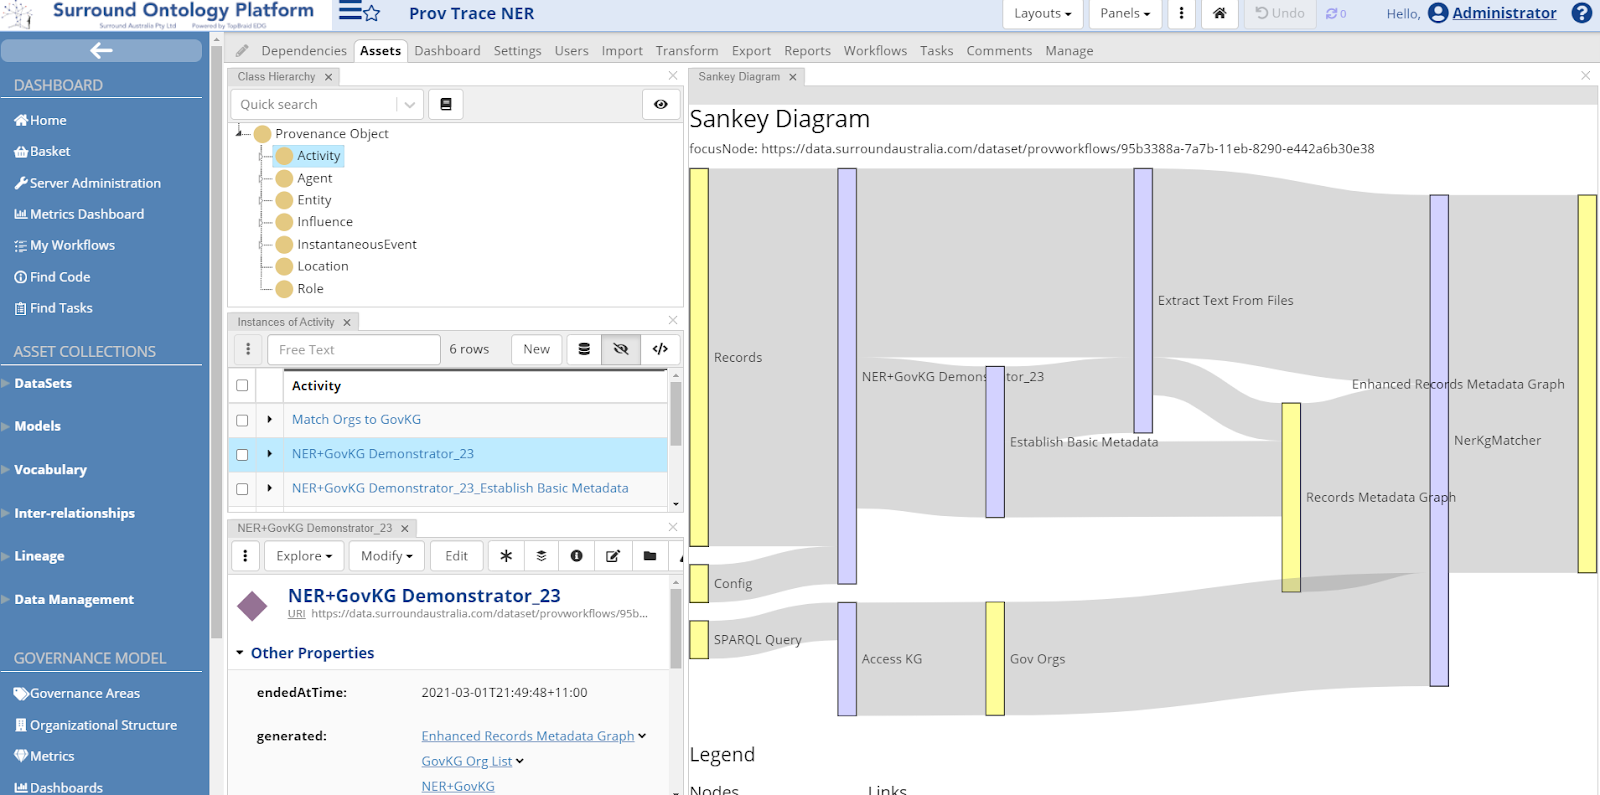
\includegraphics[width=\textwidth]{images/sankey.png}
  \end{center}
  \caption{\label{fig:sankey} An example of a provenance trace from a processing workflow that uses elements of a knowledge graph, performs processing in cloud-hosted scalable services, generates augmented views of an input stream (performing Named Entity Recognition on a document set and annotating with elements from the knowledge graph), persists the results in the knowledge graph and integrates the provenance trace with the provenance trace generated by knowledge graph management.}
  \end{figure*}
%-------------------------------------------------------------------------------

The provenance granularity issue can be addressed by examining a range of different types of processing that may typically 
occur in a heterogeneous systems and do occur within our projects. Table~\ref{tab:1} lists processing functions, examples of them and (our) required granularity. We perform a per-scenario assessment of the required provenance granlarity for projects and then, since we are using PROV everywhere,
usually employ existing tools of ours to create and store it.

\begin{table*}[t]
  \centering
  \begin{tabular}{|p{5cm}|p{5cm}|p{5cm}|}
    \hline
    \textbf{Function} & \textbf{Examples} & \textbf{Granularity}\\
    \hline
    Human-in-the-loop ML classification & Establishment of defs, Registration entities, Annotation, Classification for training & Statement, Reified statements\\ 
    \hline
    Database management, Data transformation & Making data instances sets available in a useful form & Dataset (table, spreadsheet, graph etc)\\ 
    \hline
    Query & Extraction of data subsets & Dataset, Resultset\\
    \hline
    Governance & Selecting particular datasets for use & Dataset\\
    \hline
    Bulk object processing & Indexing, classification, clustering & Whole-of-workflow\\
    \hline
    Document analysis & Making information elements in a document available to finer grained processes & Document, derived dataset\\
    \hline
    KG Management & Est'ment of state of complex, modular KGs, change tracking, support for automated updates & Graph (Dataset)\\
    \hline
  \end{tabular}
  \caption{A list of project functions, examples of them and (our) required provenance granularity}
  \label{tab:1}
\end{table*}


%-------------------------------------------------------------------------------
\section{Company-wide provenance architecture}
%-------------------------------------------------------------------------------
% SURROUND has a company-wide policy on provenance which is simple that \textit{all} project data processing 
% and system operations for clients - work on demand or services supplied - must be recorded in 
% PROV-O-compliant forms, with the exception of code and data stored in version control systems which, in all 
% instances so far, are implemented in Git\footnote{Git is a free and open source distributed version control 
% system, see \url{https://git-scm.com/}}. So far, this policy has been implemented for all our main projects' 
% systems and processes, but not for minor projects, some legacy systems or administrative support functions.

%-------------------------------------------------------------------------------
\begin{figure*}[ht]
  \begin{center}
    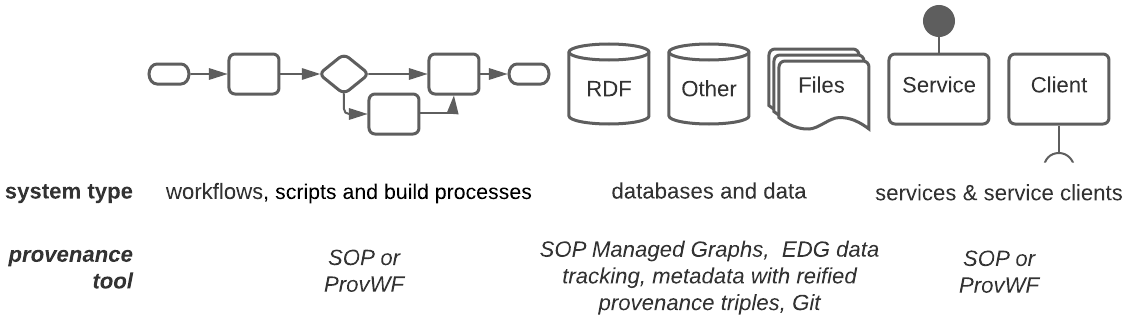
\includegraphics[width=\textwidth]{images/overview.png}
  \end{center}
  \caption{\label{fig:overview} SURROUND's provenance tools linked to system type}
  \end{figure*}
%-------------------------------------------------------------------------------

Figure~\ref{fig:overview} links types of IT project assets we work with to the tools we implement
to record PROV-O-compliant provenance. Our major provenance tools and the actions they perform are:

\begin{itemize}
  \item \textbf{SURROUND Ontology Platform} (SOP)\footnote{\url{https://surroundaustralia.com/sop}}
  \begin{itemize}
    \item an enterprise data management system based on sematic data that is based on Top Quadrant's \textit{EDG}\footnote{\url{https://www.topquadrant.com/products/topbraid-enterprise-data-governance/}}
    \item SOP extends EDG adding management of semantic asset state and collections of them
    \item SOP records PROV-DM provenance for all semantic asset actions
  \end{itemize}
  \item \textbf{ProvWorkflow} (ProvWF)\footnote{\url{https://surroundaustralia.com/provwf}}
  \begin{itemize}
    \item Python framework for creation of workflows
    \item records PROV-DM provenance for actions performed by the workflow and data consumed/produced
    \item supported by SURROUND's \textit{Block Library}
    \item itegrates with SOP by provenance bundle transfer, see Figure~\ref{fig:provwf-to-sop}
  \end{itemize}
  \item \textbf{Block Library}
  \begin{itemize}
    \item SURROUND's catalogue of ProvWF \textit{Blocks}: PROV-DM \texttt{Activity} class objects
    \item library stores many reusable functions within \textit{Blocks}, such as KG API requests, NLP text processing etc.
  \end{itemize}
  \item \textbf{Git}\footnote{\url{https://git-scm.com/}}
  \begin{itemize}
    \item to track the versions of many assets - code, data etc. - in both public and private repositories
    \item we have not yet found it necissary to materialise Git-to-PROV mappings, e.g. Git2PROV~\cite{tom_de_nies_git2prov_nodate}, but instead record URIs for entities managed in Git and refer to them in PROV-O data
  \end{itemize}
\end{itemize}

In addition to these tools, we implement provenance tracking with general-purpose tools too, such as:

\begin{itemize}
  \item \textbf{RDFlib}\footnote{\url{https://github.com/RDFLib/rdflib}}
  \begin{itemize}
    \item general-purpose Python RDF manipulation library
    \item many of our data objects are RDF graphs
    \item we maintain RDFlib code blocks, e.g. to create reified provenance for RDF statements
  \end{itemize}
\end{itemize}  

% %-------------------------------------------------------------------------------
% \begin{figure*}
%   \begin{center}
%     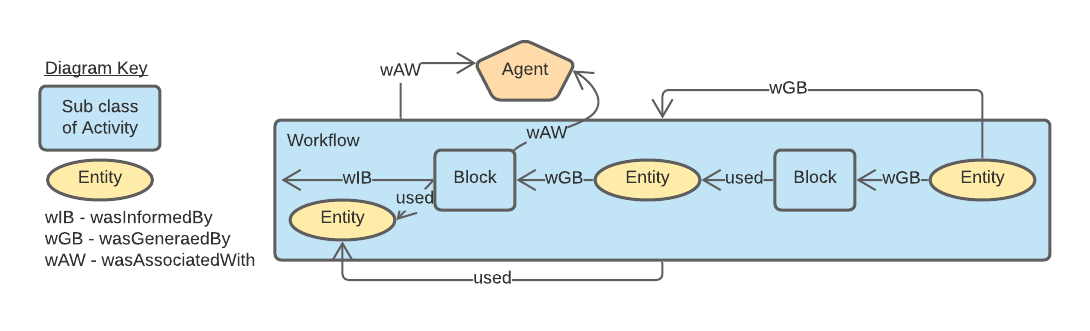
\includegraphics[width=\textwidth]{images/provwf.png}
%   \end{center}
%   \caption{\label{fig:provwf} An example of the main PROV-O elements generated by \textit{ProvWF}. Note that the tooling automatically captures identifiers for the versions of software used for any particular workflow implementatation}
%   \end{figure*}
% %-------------------------------------------------------------------------------

%-------------------------------------------------------------------------------
\begin{figure*}[ht]
  \label{fig:provwf-to-sop}
  \begin{center}
    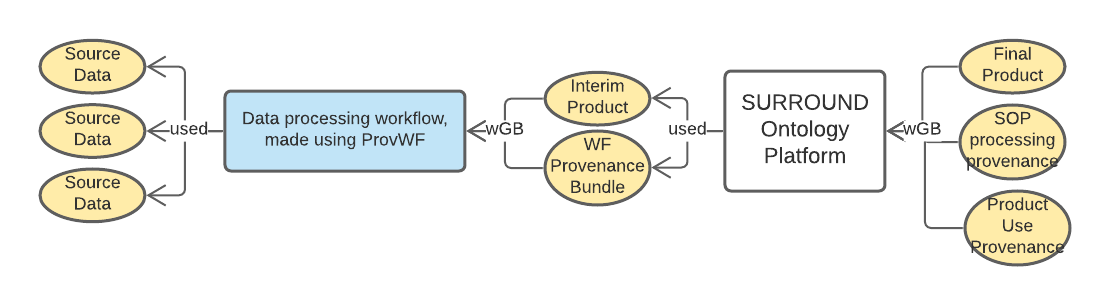
\includegraphics[width=\textwidth]{images/provwf-to-sop.png}
  \end{center}
  \caption{\textit{ProvWF} is often used to generate RDF data - here the ``Interim Product'' - which can be supplied to \textit{SOP} with an acompanying provenance \texttt{Bundle}. \textit{SOP}, in turn, generates both \texttt{Bundles} of provenance for any actions on data it performs and also records usage provenance for products}
\end{figure*}
%-------------------------------------------------------------------------------

%-------------------------------------------------------------------------------
\section{Aspects of our provenance modelling}
%-------------------------------------------------------------------------------
Much of our provenance modelling will be familiar to PROV users: chains of \textit{Activities} and \textit{Entities} associated with 
\textit{Agents}. We do have several project scenarios which cause us to implement slight specialisations and two are given in project-
specific case studies next.

\subsection{Project 1: Electronic Records assessment}
A recent project of ours has applied Natural Language Processing and KGs to electronic Records classification for archiving: we have extracted elements of Records' content, compared them with managed sources of \textit{context} presented as KGs and used ML to learn
how best to classify the Records.

Important in this project's provenance capture has been the use of data services - our classification workflow system querying our own
KG services - and the tracking of both whole-workflow and individual data statement provenance. Figure~\ref{fig:reified-graph-data} shows our 
model for data service query tracking within a workflow. Whole-of-workflow provenance is needed to track what configurations produce what 
results. All of the instances of a workflow's execution and the individual elements within it are recorded as PROV \texttt{Activity} instances
and data as PROV \texttt{Entities}.  
Individual data statement provenance is needed for classifications within a Record's medata in RDF so individual Record results can 
be verified. Workflow, metadata and metadata provenance are all stored in an RDF database and are crosslinked.

%-------------------------------------------------------------------------------
\begin{figure*}
  \begin{center}
    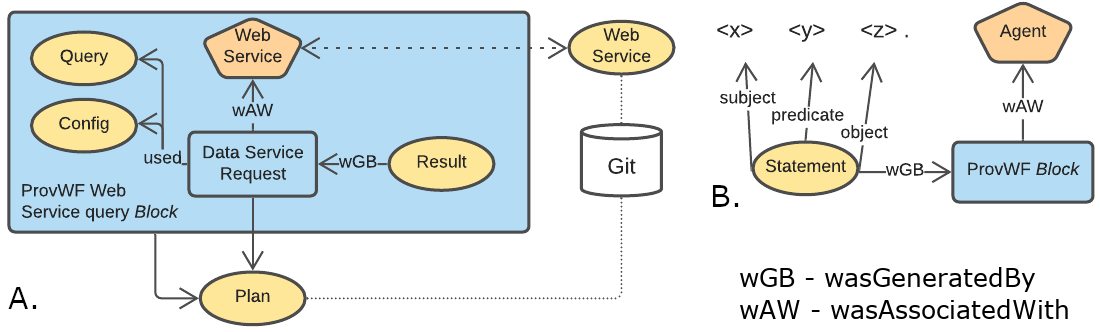
\includegraphics[width=\textwidth]{images/ds-reified.png}
  \end{center}
  \caption{\label{fig:reified-graph-data} \textbf{A}. A \textit{Service query block} from our \textit{Block Library}, implemented within our \textit{ProvWF} framework using a Query and other configuration (Config) to query a Web Service agent for a Result. Provenance for the web service itself, now considered an entity, is recorded in Git systems and referenced by each \textit{ProvWF} execution. \textbf{B}. Reified provenance for a single RDF triple associated with the \textit{ProvWF} Block instance that generated it.}
\end{figure*}
%-------------------------------------------------------------------------------

Since shortly after the publication of PROV, SURROUND has watched extensions to it, or specialisations of it, for workflows. Our workflow modelling 
follows fairly simple PROV extensions such as PROV-Wf \cite{costa_2013} however, we find that the \texttt{Plan},
or instructions for workflow execution are naturally recorded within the workflow's defining software
code, so our \textit{ProvWF} tool records a URI reference to the version of the code (the Git \textit{commit} or \textit{release}) that was executed.
\textit{ProvWF} requires custom PROV-style logging to be defined per custom \textit{Block}, unless pre-defined \textit{Block} instances from our 
\textit{Block Library} are used. We have considered systems that generate PROV-compatable workflow provenance more automatically from defined 
workflow elements, such as \cite{prabhune_prov2one_2016} but have, so far, found that the level of workflow specification needed for those approaches 
(using a specialised business process modelling language) exceeds the provenance granularity we need for our workflows and forces us to simple define 
non-executable data structures as complex as simple directly defining PROV itself (perhaps more so).

Some recent work on scientific workflow provenance \cite{butt_provenance_2021} focus on modelling control flow to 
answer questions such as ``what are the reasons for divergent results in two executions of a workflow?''. Currently we do not implement such 
modelling in \textit{ProvWF} or any other tool and instead represent workflows only as a simple \textit{Workflow} containing \textit{Blocks} that are 
arranged liniarly in time: all control flow decision making is subsumed into \textit{Blocks} which does make them complex, but, so far, we have been 
able to model all interesting control flow choices as \textit{Block} inputs or outputs. If, in future projects, we are interested to further focus on
particular workflows' control flow elements, we anticipate representing them as a specialised \textit{Block} with templated (expected) inputs and 
outputs and then comparing instances of that specialised \textit{Block} to discover control flow choices.

\subsection{Project 2: Document semantic querying}
Another project of ours involved decomposing a large industry specification document into not only structural but also semantic elements (phrase
meanings, synonyms, diagram descriptions, terminology lists, algorithm elements) to facilitate natural language and na\"ive searching of it. To track
the efficacy of different document content decomposition methods and of different reference datasets - vocabularies of industry-specific terms etc. - 
we implemented a multi-system proveance regime. This involved modelling datasets (often KGs) as PROV \textit{Entity} instances and tracking their 
state over time as queries were put to the multi-part system. We tracked the inbound queries to our system as per work some of our authors conducted 
many years ago \cite{car_enabling_2016} which treats each request as a PROV \texttt{Activity} from an anonymous \texttt{Agent} and for which results v. KG state are extracted from web logs.

Tracking reference dataset state in this project was done through the use of our SOP tool whcih has had graph state tracking capability added to 
it over many years and which allows for provenance about changes, new data insertions etc. to be recorded for both whole datasets within a set and 
also elements within the datasets. In SOP we can refer to the state of a collection of assets with a single URI reference - a \textit{version} of an asset collection - and the provenance of queries and workflows quote that URI to ensure provenance cross querying is possible. 

% TODO:
% first scenario
%   reference Plan use for workflow
%   cite Butt but dismiss
% second sceanrio
%   finish above section
%   any image for second scenario?

%-------------------------------------------------------------------------------
\section{Reflections on PROV modelling}
%-------------------------------------------------------------------------------
We have appreciated the graph-based nature of PROV-DM (in the PROV-O form that we use it) and find this aspec of PROV, along with the RDF methods for
object identification and extensible schemas, to be the most useful aspect of PROV. These alow us to model ``anything'' at any level of granularity,
store provenance data in one kind of system and cross query it to dive into elements, aggregate values etc.

Few aspects of PROV have been problematic for us but those that have include:

\begin{enumerate}
  \item difficulty in storing a complex data in provenance graphs
  \begin{itemize}
    \item when we wish to store complex objects for provenance but don't want to persist them in data store seperately to provenance KGs, we have struggled to think of how to represent them, without resorting to excruciating Semantic Web modelling
  \end{itemize}
  \item linking \texttt{Entity} instances to \texttt{Plane} instances
  \begin{itemize}
    \item we want to be able to associate PROV \texttt{Entity} instances to the \texttt{Plan} instances used to instruct the workflows that generated them. PROV struggles to allow persstent \texttt{Entity} / \texttt{Plan} relations
  \end{itemize}
\end{enumerate}  

%-------------------------------------------------------------------------------
\section{Conclusions}
%-------------------------------------------------------------------------------
SURROUND uses fairly standard patterns with PROV to model provenance across multiple systems and within different IT domains.
We have easily adapted the PROV model to provide provenance that gives our customers confidence in the results
they receive from us via access to individual results' lineage, particularly important for complex AI/ML applications, and gives us the 
ability to learn how our multi-part systems perform against tasks through cohesive logging. We have put considerable effort into establishing
technical interfaces, interactions and integrations between our tools. We have developed both dedicated provenance tools and provenance
capability within generic tools. We have not, so far, had to use highly specialised versions of PROV to achieve our goals.

%-------------------------------------------------------------------------------
\bibliographystyle{plain}
% \bibliography{\jobname}
\bibliography{TaPP21}

%%%%%%%%%%%%%%%%%%%%%%%%%%%%%%%%%%%%%%%%%%%%%%%%%%%%%%%%%%%%%%%%%%%%%%%%%%%%%%%%
\end{document}
%%%%%%%%%%%%%%%%%%%%%%%%%%%%%%%%%%%%%%%%%%%%%%%%%%%%%%%%%%%%%%%%%%%%%%%%%%%%%%%%

%%  LocalWords:  endnotes includegraphics fread ptr nobj noindent
%%  LocalWords:  pdflatex acks
